% Native TeX feature showcase — demonstrates the two capabilities added by
% the native-TeX text engine (desktop only, requires latex + dvisvgm + a
% Ghostscript install for \includegraphics):
%
%   1. \includegraphics inside a node renders the actual image
%   2. User-defined preamble macros (\newcommand, \def, \DeclareMathOperator)
%      expand correctly in node text — MathJax would silent-fail on these
%
% Open this file from the desktop app. Each figure below is separately
% draggable + editable; the underlying rendering path is chosen per node.

\usepackage{amsmath}
\usepackage{amssymb}
\usepackage{xcolor}

% User-defined macros — the preamble is threaded into every native compile,
% so any node text mentioning one of these routes through native TeX.
\newcommand{\bfheading}[1]{\textbf{\large #1}}
\newcommand{\emphred}[1]{\textbf{\color{red}#1}}
\newcommand{\R}{\mathbb{R}}
\newcommand{\myVec}[1]{\boldsymbol{#1}}
\newcommand{\inner}[2]{\langle #1, #2 \rangle}

\DeclareMathOperator{\argmax}{arg\,max}
\DeclareMathOperator{\Var}{Var}

\def\halfway{0.5}


% ── Figure 1 ─────────────────────────────────────────────────────────────
% Text macros. \bfheading + \emphred are user-defined so MathJax cannot
% expand them — routing catches the macro names, sends the fragment to
% native TeX, which has the preamble in scope.

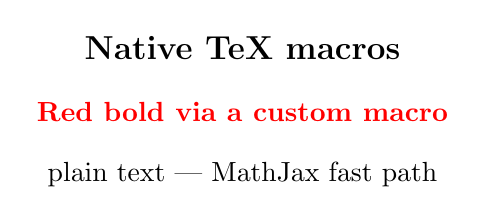
\begin{tikzpicture}
  \node at (0, 0.8)  {\bfheading{Native TeX macros}};
  \node at (0, 0)    {\emphred{Red bold via a custom macro}};
  \node at (0, -0.8) {plain text — MathJax fast path};
\end{tikzpicture}


% ── Figure 2 ─────────────────────────────────────────────────────────────
% Math macros. Every fragment references \myVec / \R / \argmax / \Var /
% \inner / \halfway, so every node routes to native TeX. The compile
% wraps each fragment with the preamble above.

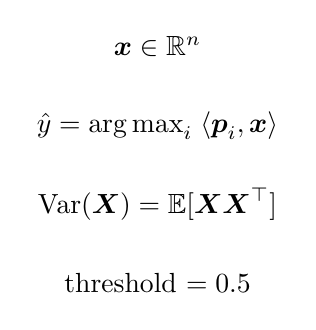
\begin{tikzpicture}
  \node at (0, 1.5)  {$\myVec{x} \in \R^n$};
  \node at (0, 0.5)  {$\hat{y} = \argmax_i \; \inner{\myVec{p}_i}{\myVec{x}}$};
  \node at (0, -0.5) {$\Var(\myVec{X}) = \mathbb{E}[\myVec{X}\myVec{X}^\top]$};
  \node at (0, -1.5) {threshold $= \halfway$};
\end{tikzpicture}


% ── Figure 3 ─────────────────────────────────────────────────────────────
% \includegraphics inside a node. Requires a TeX distribution + Ghostscript
% (the app auto-detects both on macOS/Linux/Windows). The image is loaded
% from the same directory as this .tex file.

\begin{tikzpicture}
  \node[label=below:{$\sin x$}] at (0,0)   {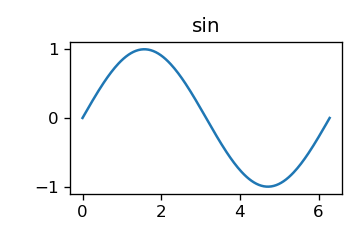
\includegraphics[width=3.5cm]{plot_sin.png}};
  \node[label=below:{contour}]  at (5,0)   {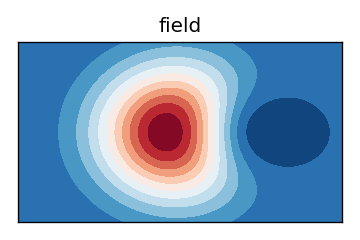
\includegraphics[width=3.5cm]{plot_contour.png}};
\end{tikzpicture}


% ── Figure 4 ─────────────────────────────────────────────────────────────
% Everything combined: an image, a macro-typeset annotation, and a
% standard TikZ arrow between them. Three rendering paths in one picture.

\begin{tikzpicture}
  \node[inner sep=0pt] (plot)  at (0,0)   {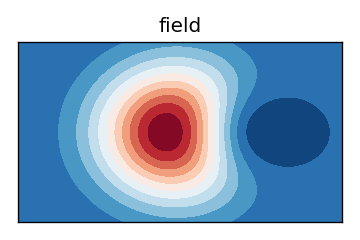
\includegraphics[width=4cm]{plot_contour.png}};
  \node                (label) at (5.5,0) {\emphred{peak at $\argmax$}};
  \draw[->, thick, red] (label.west) -- (0.6, 0.3);
\end{tikzpicture}
